\bartchapterimage{sdss}
\bartthumb{thumb_sdss}
\cs{Analysing SDSS-DR8\label{ap:sdss}}

% une mini table des matières
%\minitoc%

\fs{Introduction}

In order to realize the mock catalogue for the group finder algorithm, we need to mimic the SDSS. This mock have to be realistic.
But our algorithm needs to have the redshift for \emph{all} galaxies in the volume selected and the SDSS provides spectroscopic
redshifts just for galaxies that could have been targeted due to the problem of fibre collision. So for galaxies in this situation
we use the photometric redshift. The problem is that dense regions on the survey are more susceptible to don't have a spectroscopic
redshift than a galaxy in a lower dense region. So we have to determine how the fraction of photometric galaxies depends on the
density of galaxies in the sky in order to apply this in our mock catalogue.

In the SDSS, there are different ways to estimate photometric so we list the methods here. \com{Add the list of method available in
the SDSS}.

We can select galaxies in the sample with an SQL query. All queries used will be summary here.

\begin{wrapfigure}{r}{0.5\linewidth}
    \centering
    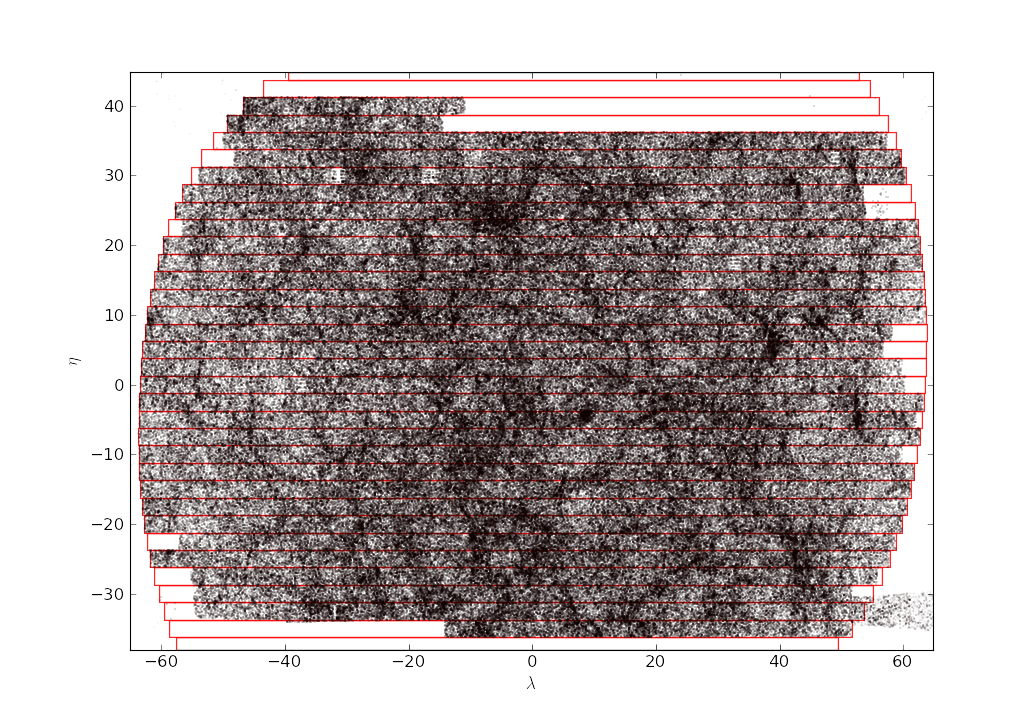
\includegraphics[width=\linewidth]{SpectroGalStripesSDSSoriginal.png}
    \caption{\footnotesize{}Spectroscoped galaxies in the SDSS DR8 with stripes limits as planned. Coordinates are in degrees.}
    \label{fig:SDSSspecgalstripes}
\end{wrapfigure}
\fs{Analysis}
\fss{Definitions}

In the SDSS there is something called "stripes" which is a band of observations in the sample. Those \emph{bands} can overlap
contrary to "chunks" which are similar bands but don't overlapping (they make a complete partition of the survey in their union). We
can use this stripes in order to select galaxies in regions of interest for our studies. Data on the SDSS provide limits of this
stripes, so we can use it to fix borders of the survey. In reality, in the region of the survey we consider, we don't see
overlapping of the stripes. So it is more useful to use them in order to define limits of survey in region of our interest.

Following definitions given in the SDSS website, we can define two other coordinate systems in the survey which we can use to select
galaxies.
\begin{description}
	\item[Great Circle:] This coordinates system is define with two angle $(\mu, \nu)$. Coordinates are relatives to one stripe
	so it can be use when working with galaxies in the region of the stripe we consider. \com{More definitions of this}.

	\item[Survey Coordinates:] It's an other system similar to celestial coordinates but "centred" on the "block" of galaxies of
	the survey that we can see in maps. Coordinates are written $(\eta,\lambda)$. If we use celestial coordinates, we have:
	\begin{eq}
	        (\num{0},\num{90}°)_{(\eta,\lambda)}=(\num{275}°,\num{0})_{(\alpha,\delta)}\;\;\;\;
	        (\num{57.5}°,\num{90}°)_{(\eta,\lambda)}=(\num{0},\num{90}°)_{(\alpha,\delta)}
	\end{eq}
	It results from this that $-\cfrac{\pi}{2}<\eta<\cfrac{\pi}{2}$ and $-\pi<\lambda<\pi$.
\end{description}

Wee this informations we can write the transformations between the different coordinate systems.
\fsss{Survey coordinates to celestial coordinates}
From previous definitions, we see that the relation between those systems is just a rotation. So:
\begin{eqnarray}
        \delta &=& \arcsin\pg\cos\lambda\sin\pg\eta+32.5°\pd\pd\nonumber\\
        \alpha &=& \mathrm{atan2}\pg\sin\lambda,\cos\lambda\cos\pg\eta+32.5°\pd\pd+185°\nonumber\\
\end{eqnarray}

\fsss{Celestial coordinates to survey coordinates}
The inverse transformation is in consequence:
\begin{eqnarray}
        \eta &=& \mathrm{atan2}\pg\sin\delta,\cos\delta\cos\pg\alpha-\alpha_0\pd\pd-\delta_0\nonumber\\
        \lambda &=& \arcsin\pg\cos\delta\sin\pg\alpha-\alpha_0\pd\pd\nonumber\\
\end{eqnarray}
with $(\alpha_0,\delta_0)_{(\alpha,\delta)}=(0,0)_{(\eta,\lambda)}$.
We have to apply too periodic conditions in the angles founded by the latter equation in order to have values in the correct range.
So conditions are:
\begin{eqnarray}
        \mathrm{Where}&\;& \eta<-\num{90}°\;\mathrm{or}\; \eta>\num{90}°:\nonumber\\
        & & \eta\rightarrow\eta+\num{180}°\nonumber\\
        & & \lambda\rightarrow\num{180}°-\lambda\nonumber\\
\end{eqnarray}
\begin{eqnarray}
        \mathrm{Where}&\;& \eta>\num{180}°:\nonumber\\
        & & \eta\rightarrow\eta-\num{360}°\nonumber\\
\end{eqnarray}
\begin{eqnarray}
        \mathrm{Where}&\;& \lambda>\num{180}°:\nonumber\\
        & & \lambda\rightarrow\lambda-\num{360}°\nonumber\\
\end{eqnarray}

Determining the number of a stripe to which a galaxy pertains is easy too because stripes are organized such they have a constant
width along the $\eta$ coordinate, with a width of \num{2.5}°. The number of the stripe $n$ of a galaxy with $\eta$ position is:
\begin{eq}
        n = \mathrm{floor}\pg\cfrac{\pg\eta+\num{58.75}°\pd}{\num{2.5}°}\pd
\end{eq}

\fss{Galaxies selection}
There are many tables in the SDSS saving galaxies and other objects properties extracted from images of the survey. Those tables are
the results of different selections in objects detected in images. . When crossing objects between images of the survey that
overlap, there are some differences of positions between the same object in the two images. So there are possibilities that an
object is observed twice or more. In many of those tables, there is no "double objects".

The \texttt{Galaxy} view is a selection from the \texttt{PhotoPrimary} for objects flagged as \emph{galaxy}. The \texttt{Galaxy}
view contains the photometric parameters (no redshifts or spectroscopic parameters) measured for resolved primary objects. But we
have other useful informations to link with tables that give us photometric and spectroscopic redshifts. There is the
\texttt{specobjid} to link with spectroscopic redshifts in the table \texttt{SpecObj} which doesn't contain duplicates (it's a clean
table of \texttt{SpecObjAll} with clean redshifts). If \texttt{specobjid=0}, the galaxy doesn't have a spectroscopic redshift. The
\texttt{objid} is a link to the \texttt{Photoz} table which contains all photometric redshifts for galaxies in the \texttt{Galaxy}
table. Estimation is based on a robust fit on spectroscopically observed objects with similar colors and inclination angle. There is
also the \texttt{PhotozRF} where estimates are based on the Random Forest technique. Galaxies in the \texttt{SpecObj} are limited to
$m_r<17.77$ and a surface brightness selection \com{Add This !!}. So we need to do the same flux limitations when selecting galaxies
on the \texttt{Galaxy} table. A possible SQL query for selecting galaxies in this table and link them with redshifts tables could
be for spectroscoped galaxies:
\begin{listing}[H]
\begin{minted}[bgcolor=griscode, linenos]{sql}
select GG.ra, GG.dec, GG.petroMag_u, GG.petroMag_g, GG.petroMag_r,
GG.petroMag_i, GG.petroMag_z, GG.specobjid, GG.objid, Z.z, Z.Zerr
from Galaxy as GG, SpecObj as Z
where Z.specobjid=GG.specobjid and GG.specobjid!=0 and GG.petroMag_r<17.77
and GG.ra<275 and GG.ra>100 and GG.dec>-10 and GG.dec<75
\end{minted}
\end{listing}
\noindent and for galaxies which couldn't be spectroscoped:
\begin{listing}[H]
\begin{minted}[bgcolor=griscode, linenos]{sql}
select GG.ra, GG.dec, GG.petroMag_u, GG.petroMag_g, GG.petroMag_r,
GG.petroMag_i, GG.petroMag_z, GG.specobjid, GG.objid, Z.z, Z.Zerr
from Galaxy as GG, Photoz as Z
where GG.specobjid=0 and GG.objid=Z.objid and GG.petroMag_r<17.77
and GG.ra<275 and GG.ra>100 and GG.dec>-10 and GG.dec<75
\end{minted}
\end{listing}

Limits of stripes are given in the SDSS table \texttt{StripeDefs} but this limits aren't actual limits, they are planned limits when
survey started. We can see it on the figure(\ref{fig:SDSSspecgalstripes}) where planned limits are shown in red and spectroscoped
galaxies are the points.

We see that some planned regions aren't still observed (spectroscopically speaking). So we need to define other limits in $\lambda$
coordinates for that stripes that aren't completes. We find by hand the new limits of stripes which contains spectroscoped galaxies.
Now, the survey mask is like in figure(\ref{fig:SDSSspecgalstripesnew}). We will consider just galaxies in this mask in order to
find groups in the SDSS. Other galaxies aren't easy in order to define borders of the survey and find groups.
\begin{figure}[ht]
	\centering
	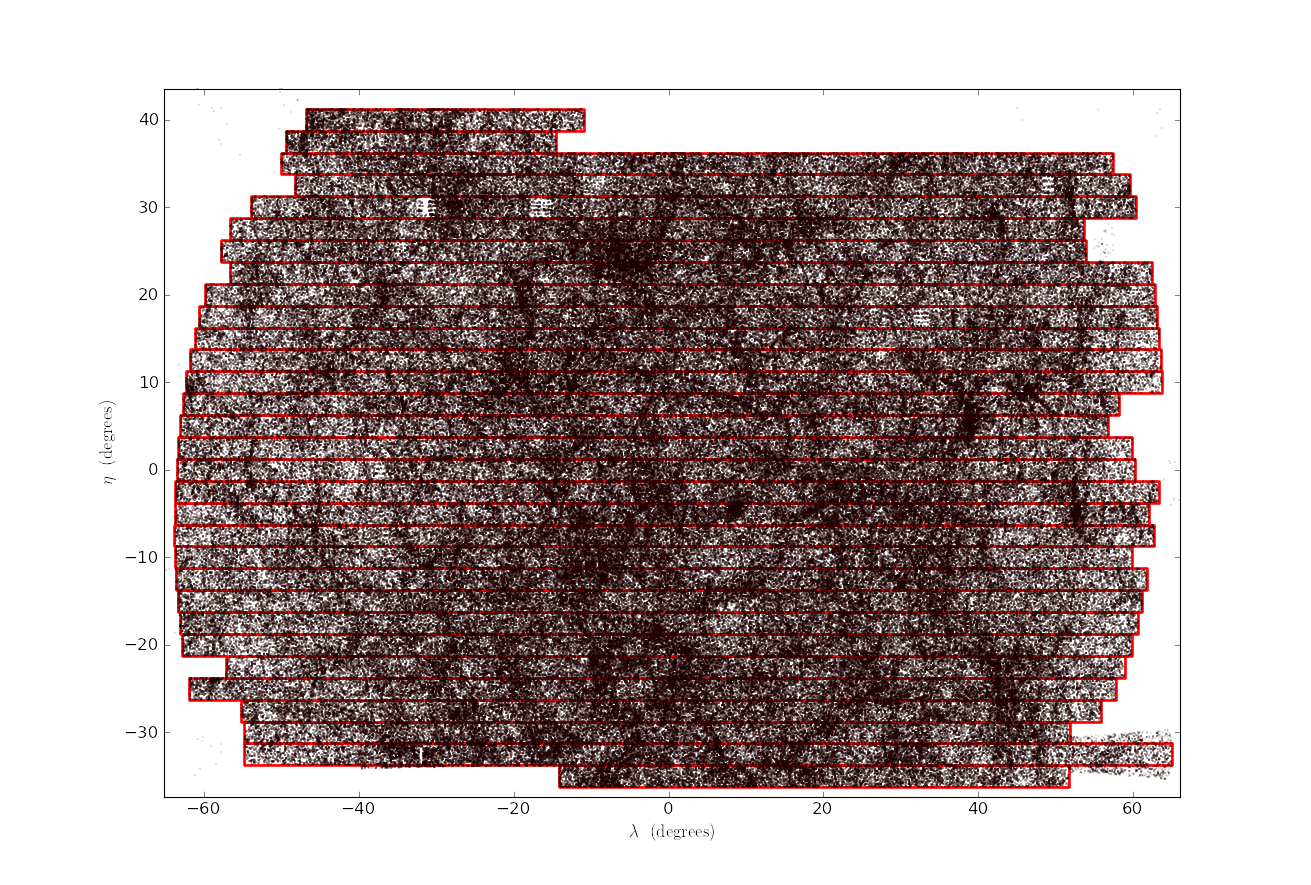
\includegraphics[width=\linewidth]{SpectroGalStripesSDSSnew.png}
	\caption{\footnotesize{}Spectroscoped galaxies in the SDSS DR8 with stripes limits chosen in order to find easily groups at
	the border of the survey.}
	\label{fig:SDSSspecgalstripesnew}
\end{figure}

For fibre collisions galaxies, we use galaxies selected in the table of the photometric redshifts and keep galaxies that are in the
mask defined previously. Now we have a sample of galaxies in a region of the SDSS for which we can easily characterize borders and
where all galaxies, given the flux limit of the SDSS, are presents. There is just the problem of fibre collisions galaxies for which
the redshift in our possession is photometric, in consequence less precise than spectroscopic redshifts. But our algorithm is tested
on a mock catalogue which is "perfect" if we don't take in account this problem of less robust photometric redshifts. In order to
know the behaviour of the algorithm with those problematic redshifts, we need to implement this in our mock catalogue.

\fsss{Flags in the SDSS}

Galaxies can have some troubles with photometry, resolve etc... due to fit and estimations in the SDSS. in the general case, those
objects are flagged with the \texttt{clean} property which indicates by \num{1} that the photometry is OK and by \num{0} when there
is a problem. Details of the problems are in the bit flag. But for groups, we need to select all galaxies, whether there are not
clean.

\texttt{Galaxy} table is a selection from \texttt{PhotoPrimary} view for objects with $\mathrm{\texttt{type}}=3$ (galaxy). I think
that we don't have to care of the "good" photometry of galaxies in the \texttt{Galaxy} view, but we can leave a flag in the group
finder algorithm to say if a galaxy is in this case.

However, we have to take into account the error on the redshift estimation using the \texttt{zErr}. For photometric redshift I think
that if the \texttt{zErr} is too high, we can use the \texttt{nnAvgZ} which is the average redshift of galaxies in the neighbourhood
of the considered galaxy. It can be better too if the photometric redshift is too different from it.

The \texttt{SpecObjAll} contains duplicates and bad datas. But the \texttt{SpecObj} contains just clean spectras. We use
\texttt{zWarning} to decide if we keep the redshift (\texttt{zWarning}=0) or not. In the latter case, we use the photometric
redshift instead.

\fss{Fibre collision estimation}
In the SDSS, obtaining spectroscopic redshifts of galaxies is done using a plate of \num{1.5}° diameter, in which there is a certain
number of fibres in order to get spectrum of the galaxy. But in the field of the plate, the number of fibres is limited, and the
number of coverings of a portion of the sky is limited too because of the time needed to obtain a spectrum. Although runs may
overlap, there is sometime galaxies that can't be spectroscoped. Moreover, fibres have a dimension of \num{55}'', so when galaxies
are closer than this size, one (or more) of those galaxies aren't spectroscoped. We can see that in the figure(\ref{fig:angreddist})
where we have taken the nearest neighbour of a galaxy and determined the differences in angular size and redshift between the two
galaxies. As expected, the number of galaxies which are closer than \num{55}'' decreases dramatically. There are still some galaxies
because the overlapping of runs can permit to get redshifts for galaxies behind this limit.
\begin{figure}[ht]
	\centering
	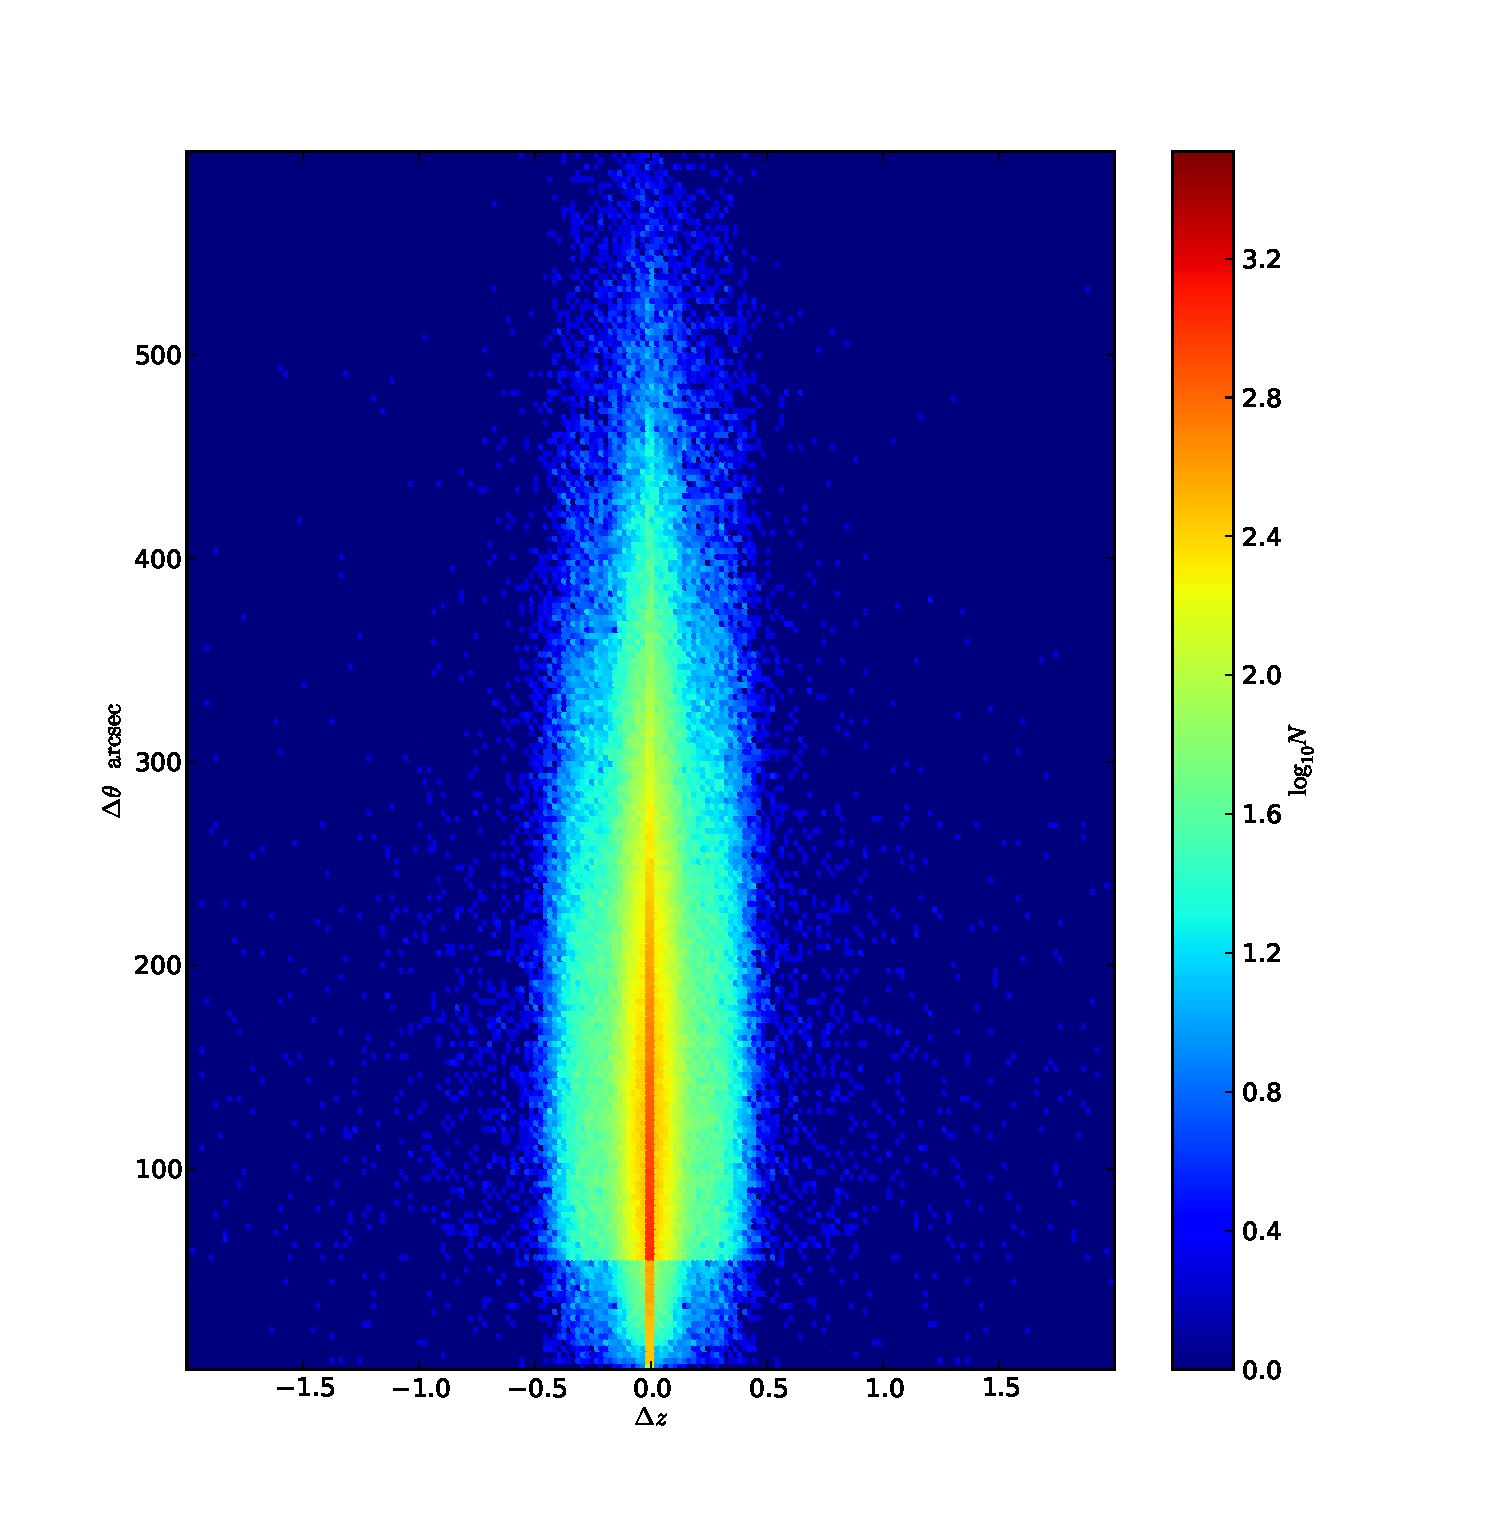
\includegraphics[width=0.6\linewidth]{distredSDSSDR8}
	\caption{\footnotesize{}Distribution of spectroscoped galaxies in the SDSS DR8 in angular size and redshift differences with
	the nearest neighbour galaxy.}
	\label{fig:angreddist}
\end{figure}

A consequence of those problems is that in denser regions, the number of fibre collision increases, affecting more our groups
analysis because the number of photometric redshifts is higher in those dense regions.

We need to implement this selection effect in our mock catalogue. For that we compute the local density in the field, taking all
galaxies in the neighbourhood of \num{1.5}° of a galaxy, and in the same time, we determine the fraction of galaxies that don't have
a spectroscopic redshift. We deduce of this a relation between the density field and the fraction of fibre collisions. In the mock
catalogue, we compute the same density field and we apply the relation estimated in the SDSS sample to the mock.\com{Do it !!} We
need for each galaxy to count the fraction of non spectroscoped galaxies in a region of \num{1.5}° radius around. We have to remove
galaxies that are to close of the border of the survey, because if we don't remove those galaxies, there are some regions with
missing galaxies and the fraction estimation will be affected. The way of selecting those galaxies is to compute a circle of
\num{1.5}° around a galaxy, and if a generated point is out of the survey, the galaxy is defined as to be closer to the limits.

We can generate samples of points at an angular distance $d$ to a point of coordinate $(\alpha_0,\delta_0)$ using formulas of the
spherical triangle. If we define a triangle by the pole, the point $(\alpha_0,\delta_0)$ and the point whose we want coordinates
$(\alpha,\delta)$ denoted $M$, we can write the following relations:
\begin{eqnarray}
        \sin\pg\alpha-\alpha_0\pd&=&\cfrac{\sin{d}\sin\gamma}{\cos\delta}\nonumber\\
        \sin\delta_0\cos\gamma&=&\cos\delta_0\cot{d}-\sin\gamma\cot\pg\alpha-\alpha_0\pd\nonumber\\
\end{eqnarray}
where $\gamma$ is like a polar angle, which have all the values between 0 and $\num{2}\pi$.
So we have now:
\begin{eqnarray}
        \alpha-\alpha_0 &=& \arctan\pg\cfrac{\sin\gamma}{\cos\delta_0\cot{d}-\sin\delta_0\cos\gamma}\pd\nonumber\\
        \delta &=& \arccos\pg\cfrac{\sin{d}\sin\gamma}{\sin\pg\alpha-\alpha_0\pd}\pd\nonumber\\
\end{eqnarray}
There are problems in poles and equator with those formulas. For a $\gamma$ limit, angles can't be recovered with those formulas.
We have in those cases:\\
with $\gamma_0=\arccos\pg\cfrac{-\sin\delta_0\cos{d}}{\cos\delta_0\sin{d}}\pd$
\begin{eqnarray}
        \mathrm{Where}&\;& \delta_0-d<0\; \mathrm{and} \;\delta_0>0 \; \mathrm{and}\; \gamma_0<\gamma<2\pi-\gamma_0:\nonumber\\
        & & \delta\rightarrow-\delta\nonumber\\
\end{eqnarray}
\begin{eqnarray}
        \mathrm{Where}&\;& \delta_0+d>0\; \mathrm{and}\;\delta_0<0 \; \mathrm{and}\; \gamma_0>\gamma\;\mathrm{or}\;\gamma>2\pi-\gamma_0:\nonumber\\
        & & \delta\rightarrow-\delta\nonumber\\
\end{eqnarray}
with $\gamma_0=\arccos\pg\cfrac{\cos\delta_0\cot{d}}{\sin\delta_0}\pd$
\begin{eqnarray}
        \mathrm{Where}&\;& \delta_0+d>\cfrac{\pi}{2} \; \mathrm{and}\; \gamma_0>\gamma:\nonumber\\
        & & \delta\rightarrow\alpha+\pi\nonumber\\
        & & \alpha\rightarrow\pi-\delta\nonumber\\
\end{eqnarray}
\begin{eqnarray}
        \mathrm{Where}&\;& \delta_0+d>\cfrac{\pi}{2} \; \mathrm{and}\; \gamma>2\pi-\gamma_0:\nonumber\\
        & & \delta\rightarrow\alpha-\pi\nonumber\\
        & & \alpha\rightarrow\pi-\delta\nonumber\\
\end{eqnarray}
\begin{eqnarray}
        \mathrm{Where}&\;& \delta_0-d<-\cfrac{\pi}{2} \; \mathrm{and}\; \gamma_0<\gamma<2\pi-\gamma_0:\nonumber\\
        & & \delta\rightarrow\alpha+\pi\nonumber\\
        & & \alpha\rightarrow-\pi-\delta\nonumber\\
\end{eqnarray}

An other way to draw circles in the sphere is to consider the point for which we want to know celestial coordinates around a given
angular distance as the pole of a new coordinate system. In this system, points at given distance of our central point are just
points with $\pi/2-\delta$ and $\alpha$ running between \num{0} and $\num{2}\pi$. We now can determine cartesian coordinates of
those points in this system and apply a rotation to go from the "real" system and the system where the central point is the pole.
In the new system we have:
\begin{eqnarray}
        X'&=&r\cos\alpha'\cos\delta' \nonumber\\
        Y'&=&-r\sin\alpha'\cos\delta' \nonumber\\
        Z'&=&r\sin\delta' \nonumber\\
\end{eqnarray}
Then the rotation matrix to go from the "real" system to the new is:
\begin{eq}
        R =
        \begin{pmatrix}
		\cos\pg\cfrac{\pi}{2}-\delta_0\pd\cos\alpha_0 & \sin\alpha_0 & \sin\pg\cfrac{\pi}{2}-\delta_0\pd\cos\alpha_0 \\
		-\cos\pg\cfrac{\pi}{2}-\delta_0\pd\sin\alpha_0 & \cos\alpha_0 & -\sin\pg\cfrac{\pi}{2}-\delta_0\pd\sin\alpha_0 \\
		-\sin\pg\cfrac{\pi}{2}-\delta_0\pd & 0 & \cos\pg\cfrac{\pi}{2}-\delta_0\pd \\
        \end{pmatrix}
\end{eq}
with $\vec{X}=R\vec{X'}$ where $\vec{X}=(X,Y,Z)$. Then we have just to convert those coordinates in celestial angles using:
\begin{eq}
        \alpha=\left\{ \begin{array}{lcr}
                         -\mbox{arctan2}(Y,X)+2\pi & \mbox{if} & Y>0 \\
                         -\mbox{arctan2}(Y,X) & \mbox{else} & \\
                        \end{array}\right.\nonumber
\end{eq}
\begin{eq}
        \delta=\mbox{sign}(Z)\arccos\left(\frac{\sqrt{X^2+Y^2}}{\sqrt{X^2+Y^2+Z^2}}\right)
\end{eq}
\begin{figure}[htb]
	\centering
	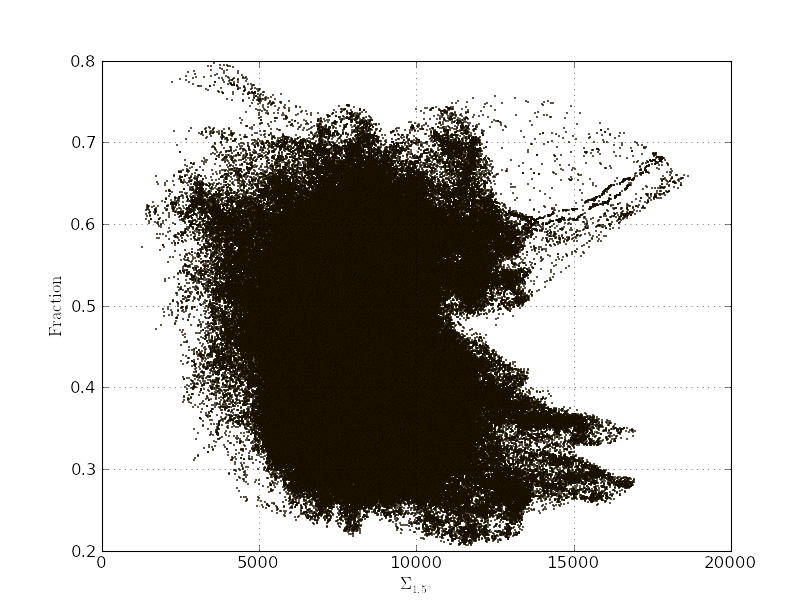
\includegraphics[width=0.6\linewidth]{FracNonSpec.png}
	\caption{\footnotesize{}Fraction of galaxies non-spectroscoped in the SDSS versus the local density field computed in a
	1.5° radius region around galaxies not to close than this radius to the border of the survey. Density is in unit of galaxies
	per degree$^2$.}
	\label{fig:fracnonspec}
\end{figure}
Fibre collisions are more probable in dense region of the sky in projection, but for the mock catalogue we need to quantify this. In
order to do that, we have selected for all galaxies in the SDSS survey as defined previously galaxies that are closer than
\num{1.5}° in angular size, which is the radius of a plate used for spectroscopy in the SDSS. With that, we can estimate the local
density field $\Sigma_{1.5°}$ in unit of number of galaxies per degree$^2$. In this selection, we can determine which galaxies had
been spectroscoped or not, and so we can estimate the fraction of non-spectroscoped galaxies. We remove for computing it galaxies
that are to close of the border of the survey, and so galaxies which are closer than the radius selected can't be used to search
neighbours because some galaxies may be missed and can affect our estimations. Results are shown in the figure
(\ref{fig:fracnonspec}).
We can't see the trend we have expected with the density field, so we thought that it can be due to the large region in which we
consider galaxies and we ran the same with a radius of \num{0.3}°. Results are in figure (\ref{fig:fracnonspec0.3}).
\begin{figure}[htb]
	\centering
	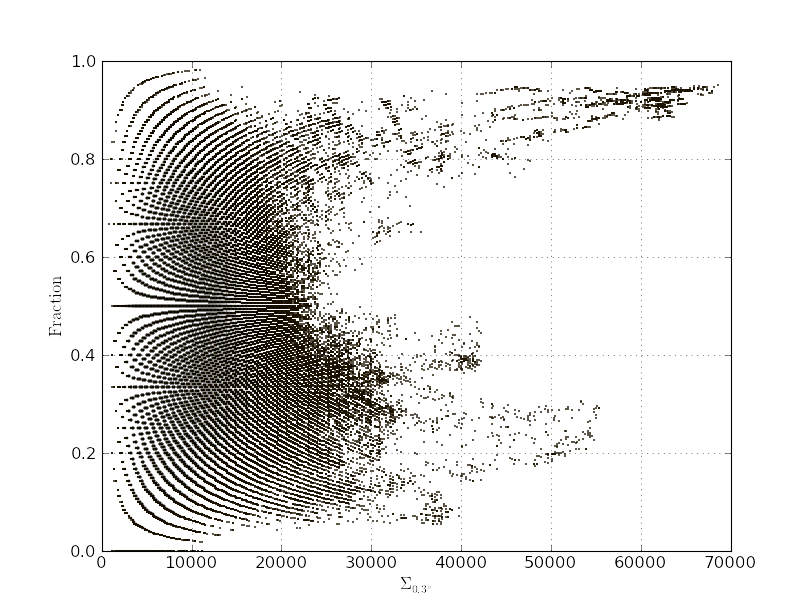
\includegraphics[width=0.6\linewidth]{FracNonSpec03.png}
	\caption{\footnotesize{}Fraction of galaxies non-spectroscoped in the SDSS versus the local density field computed in a
	0.3° radius region around galaxies not to close than this radius to the border of the survey. Density is in unit of galaxies
	per degree$^2$.}
	\label{fig:fracnonspec0.3}
\end{figure}

In order to decide which redshift to assign to a galaxy in the mock catalogue which has been chosen to have a photometric redshift,
we have estimated the distribution of photometric redshifts versus the spectroscopic redshift in the SDSS sample of spectroscoped
galaxies. Results show that a normal distribution is a well fit for those distributions, so we get for this parameters in figure
(\ref{fig:evolnormred}).
\begin{figure}[htb]
	\centering
	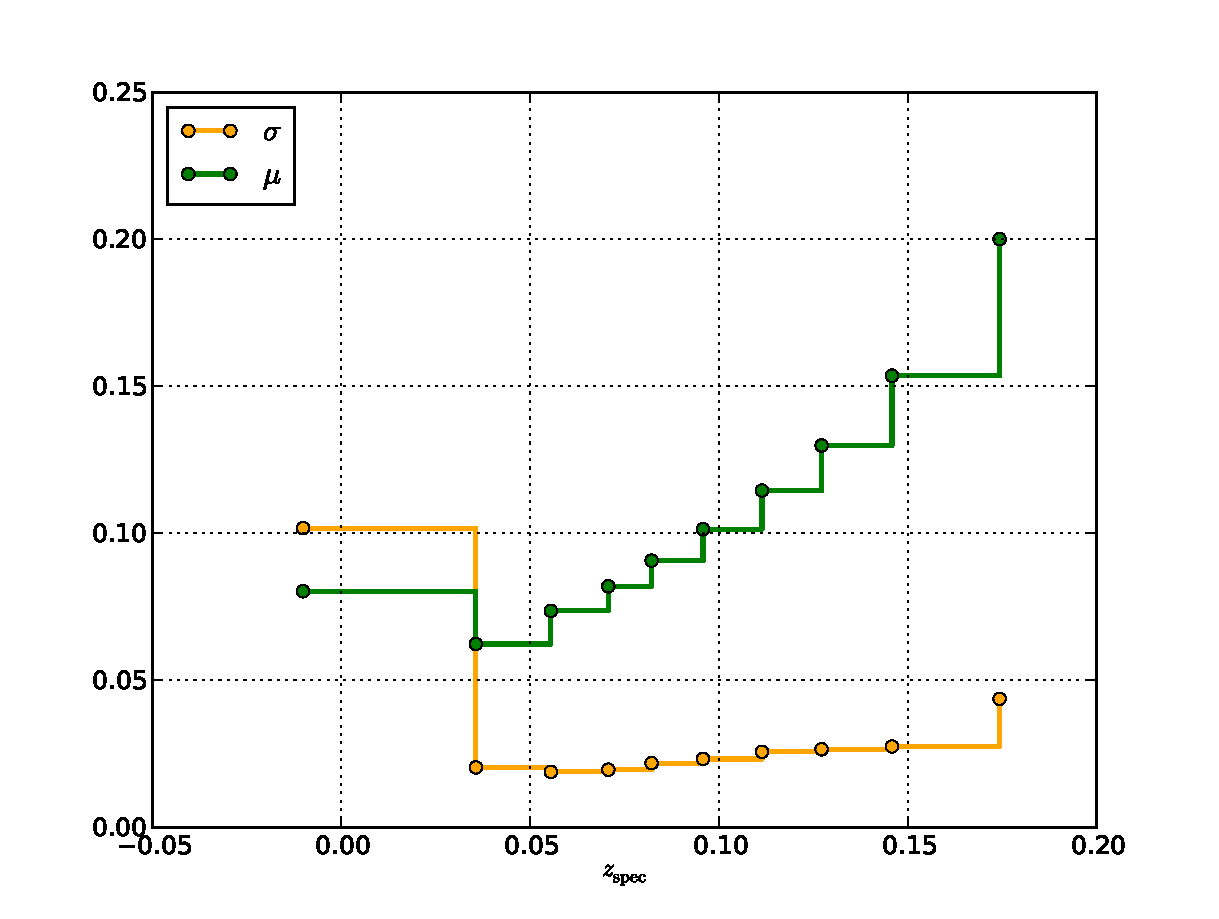
\includegraphics[width=0.8\linewidth]{EvolErrZphotSDSSDR8EqualBins}
	\caption{\footnotesize{}Parameters of a normal distribution for photometric redshifts versus spectroscopic redshifts in the
	SDSS.}
	\label{fig:evolnormred}
\end{figure}

In the mock catalogue, we have interpolated this parameters and we assign a photometric redshift for a galaxy chosen to be in fibre
collision.

\fs{Coverage of the SDSS}
For many computations in this thesis, we need to determine the surface covered on the sky by the data in our selection. The way
we have selected galaxies allows us to easily determine if a point in the sky is in our area, so we can use a Monte Carlo process
to compute this area.

First, we generate a number $N$ of points around a point of coordinates $(\alpha_0, \delta_0)$ with a maximal angular separation
$\theta_{\mathrm{max}}$ which is larger than the maximal angular separation in our sample. The fraction of those points which reside
in our selection area gives the area of the selection in fraction of the area of points generation. This area is just
$2\pi\pg1-\cos\theta_{\mathrm{max}}\pd$. \comments{I think I don't have squared angles in the expression of the solid angle.}. I
have made this calculation for different cone angle $\theta_{\mathrm{max}}$ and for different number of points to see if we have a
convergence in the value of the area. Results are shown on figure (\ref{fig:sdss_area}).
\begin{figure}[htb]
	\centering
	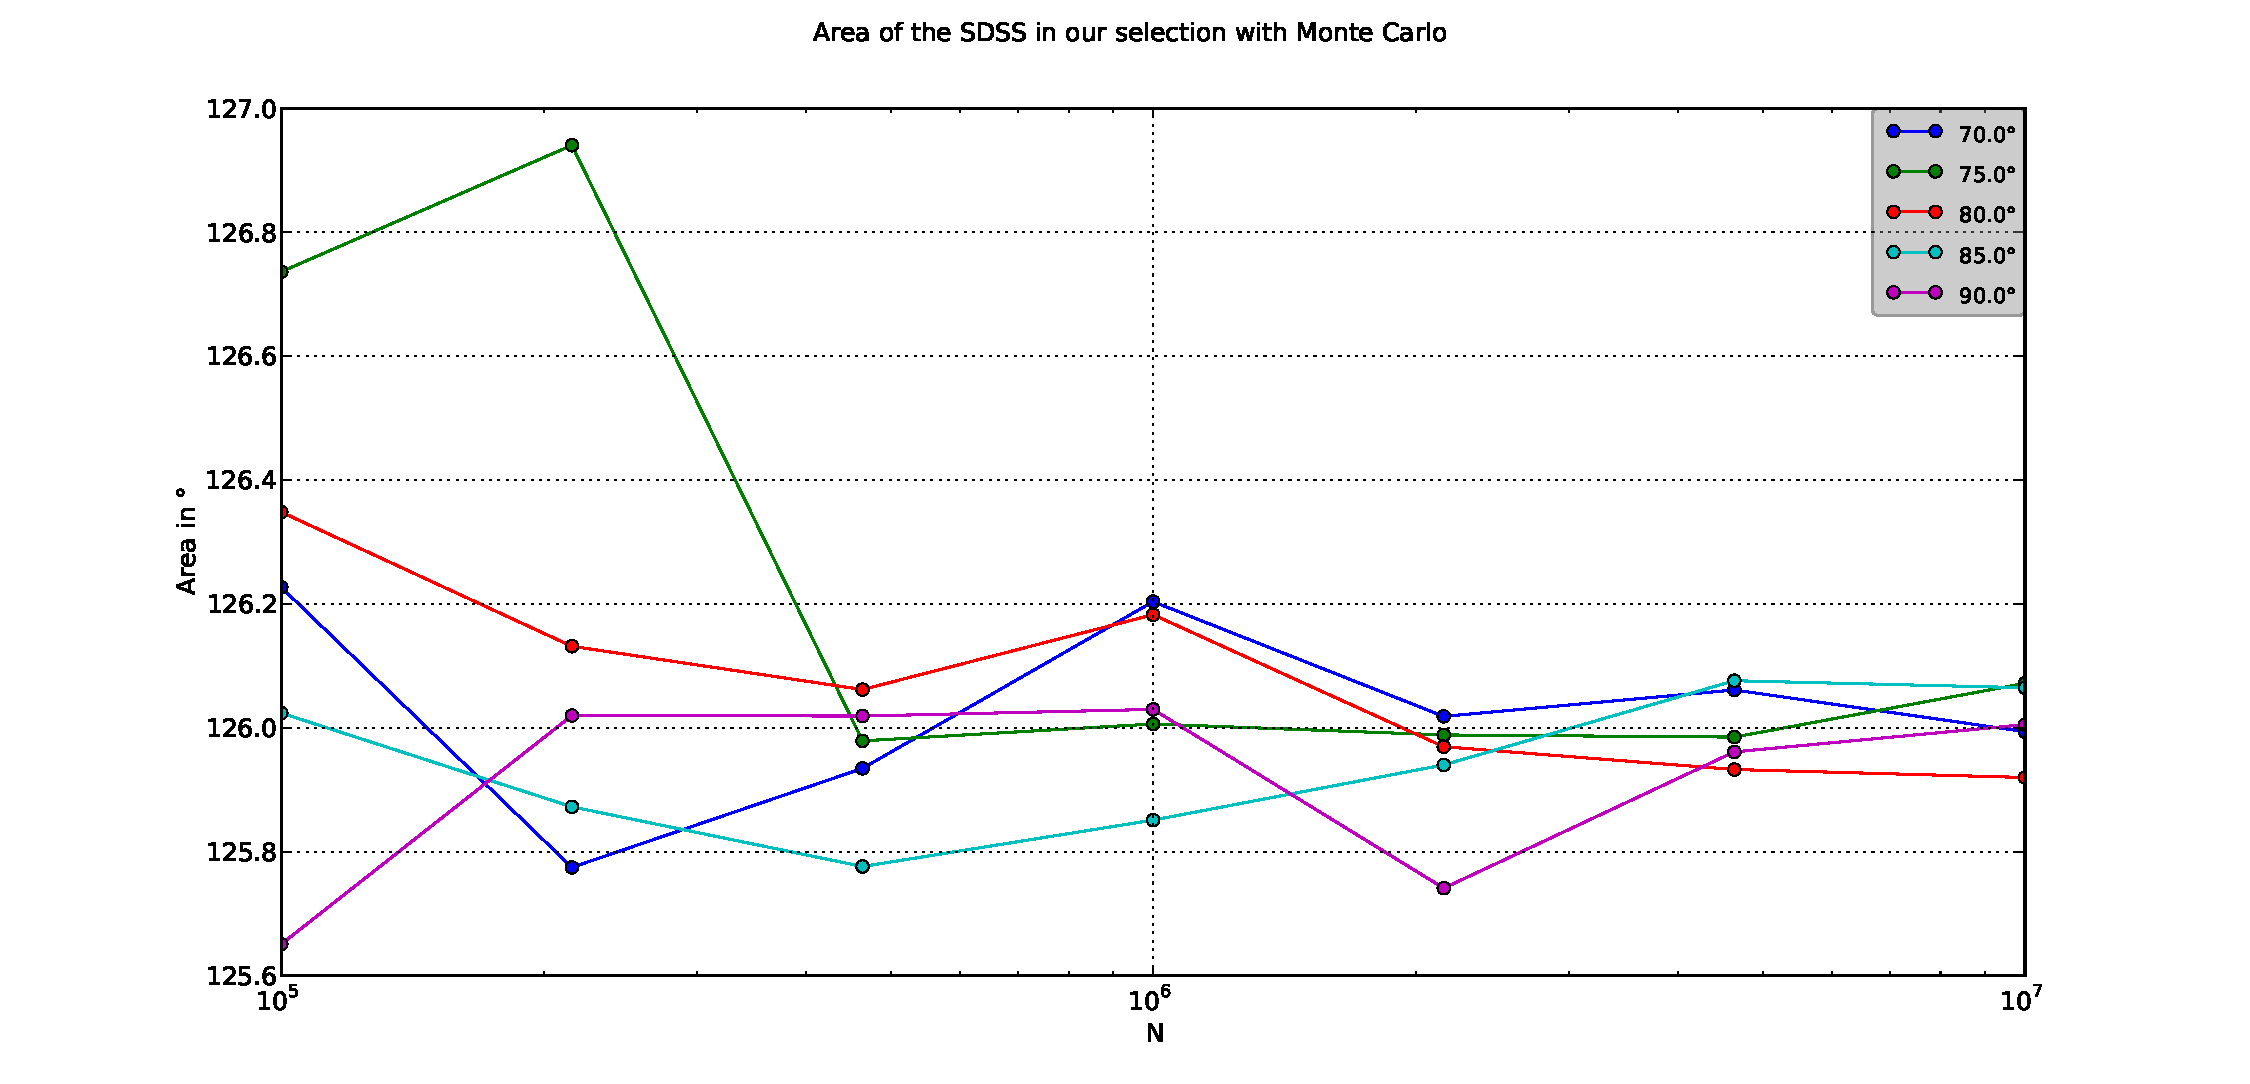
\includegraphics[width=\linewidth]{SDSS_area}
	\caption{\footnotesize{}Determination of the area of the SDSS for our selection with a Monte Carlo process. Results seem
	to converge on a value of \num{2.1993} steradians.}
	\label{fig:sdss_area}\end{figure}
